%%%%%%%%%%%%%%%%%%%%%%%%%%%%%%%%%%%%%%%%%%%%%%%%%%%%%%%%%%%%%%%%%%%%%%%%%%%%%%%%
\section{Results of the Systematic Literature Review}
\label{sec:results}
%%%%%%%%%%%%%%%%%%%%%%%%%%%%%%%%%%%%%%%%%%%%%%%%%%%%%%%%%%%%%%%%%%%%%%%%%%%%%%%%

This section presents the results of the systematic literature review conducted according to the methodology described in Section~\ref{sec:methodology}. The objective of this section is to quantitatively characterize the collected literature rather than to discuss the technical contributions of individual publications. Accordingly, the analysis focuses on the outcome of the literature search, bibliometric characteristics of the selected studies, research trends, technical topic distribution, evaluation methodologies, validation approaches, reported performance metrics, and implementation platforms. Together, these analyses provide a comprehensive overview of the current \gls{dectnr} research landscape and establish the foundation for the technical synthesis presented in Section~\ref{sec:technical_synthesis}.

%%%%%%%%%%%%%%%%%%%%%%%%%%%%%%%%%%%%%%%%%%%%%%%%%%%%%%%%%%%%%%%%%%%%%%%%%%%%%%%%
\subsection{Literature Search Results}
\label{subsec:search_results}
%%%%%%%%%%%%%%%%%%%%%%%%%%%%%%%%%%%%%%%%%%%%%%%%%%%%%%%%%%%%%%%%%%%%%%%%%%%%%%%%

The systematic literature search was performed in July~2026 following the review protocol presented in Section~\ref{sec:methodology}. Five major scientific databases, namely IEEE Xplore, Scopus, ACM Digital Library, SpringerLink, and ScienceDirect, were systematically searched using the predefined Boolean search query. In addition, Google Scholar was employed as a complementary search engine to support backward and forward snowballing and to identify relevant publications that were not indexed in the primary scientific databases. The complete study selection process followed the \gls{prisma} 2020 framework and is illustrated in Figure~\ref{fig:prisma}.

The initial database search identified 86 potentially relevant publications, comprising 42 publications retrieved from IEEE Xplore and 44 publications indexed in Scopus. No additional publications satisfying the predefined search criteria were identified in ACM Digital Library, SpringerLink, or ScienceDirect. Google Scholar returned a substantially larger number of search results; however, these were not considered part of the primary search dataset and were instead used exclusively for citation tracking and snowballing.

After removing duplicate records using Zotero Reference Manager, the remaining publications were screened according to the predefined inclusion and exclusion criteria. The screening process consisted of title screening, abstract screening, and full-text assessment. Publications unrelated to \gls{dectnr}, papers lacking sufficient technical content, inaccessible documents, and studies outside the scope of this review were excluded. Additional relevant publications identified through backward and forward snowballing were incorporated into the final literature corpus whenever they satisfied all eligibility criteria and were not already included in the primary database search.

The final dataset comprises 51 high-quality publications together with the relevant \gls{etsi} Technical Specifications, \gls{etsi} Technical Reports, and \gls{itur} recommendations that define the \gls{dectnr} standardization framework. Collectively, these documents capture the evolution of \gls{dectnr} from its initial standardization activities through protocol design, algorithm development, hardware implementation, experimental validation, and industrial deployment. This curated dataset forms the basis for the quantitative analyses presented in the following subsections and for the comprehensive technical synthesis provided in Section~\ref{sec:technical_synthesis}.

%%%%%%%%%%%%%%%%%%%%%%%%%%%%%%%%%%%%%%%%%%%%%%%%%%%%%%%%%%%%%%%%%%%%%%%%%%%%%%%%
\subsection{Bibliometric Analysis}
\label{subsec:bibliometric}
%%%%%%%%%%%%%%%%%%%%%%%%%%%%%%%%%%%%%%%%%%%%%%%%%%%%%%%%%%%%%%%%%%%%%%%%%%%%%%%%

To obtain a comprehensive understanding of the evolution of \gls{dectnr} research, the final literature corpus was analyzed from multiple bibliometric perspectives. Unlike the subsequent technical synthesis, which examines the technical contributions of the literature, the objective of this section is to characterize the research landscape quantitatively. The analysis investigates publication trends over time, publication types, primary research contributions, technical topic distribution, evaluation methodologies, validation approaches, reported performance metrics, and implementation platforms. These statistics provide valuable insights into the maturity of the research field, the dominant research directions, and the methodological evolution of the published literature.

%%%%%%%%%%%%%%%%%%%%%%%%%%%%%%%%%%%%%%%%%%%%%%%%%%%%%%%%%%%%%%%%%%%%%%%%%%%%%%%%
\subsubsection{Publication Trends}
\label{subsubsec:publication_trends}
%%%%%%%%%%%%%%%%%%%%%%%%%%%%%%%%%%%%%%%%%%%%%%%%%%%%%%%%%%%%%%%%%%%%%%%%%%%%%%%%

Figure~\ref{fig:publication_year} illustrates the annual distribution of the publications included in this systematic literature review. The figure clearly demonstrates the rapid growth of \gls{dectnr} research since the introduction of the technology. Following the publication of the earliest standardization activities in 2020, the number of scientific publications increased steadily during the subsequent years, reflecting the growing academic and industrial interest in the technology.

The publication trend indicates three distinct phases in the evolution of the research field. The first phase (2020--2022) was characterized primarily by standardization activities, architectural design, and the establishment of the fundamental communication framework. During this period, research focused on defining the protocol architecture, physical layer, medium access control procedures, and demonstrating compliance with the \gls{imt2020} requirements. The second phase (2023) represents a transition toward implementation-oriented research, during which the availability of development platforms enabled the first experimental investigations and practical demonstrations. The third phase (2024--2026) exhibits a substantial increase in research activity, with publications expanding toward protocol optimization, localization, routing, scheduling, industrial applications, hardware implementations, and large-scale experimental evaluations.

The apparent reduction in the number of publications during 2026 should not be interpreted as a decline in research activity. Instead, it reflects the fact that the literature search was conducted during the middle of the publication year, and therefore many conference proceedings and journal articles scheduled for publication later in the year were not yet available. Overall, the observed publication trend demonstrates that \gls{dectnr} has rapidly evolved from a newly standardized radio interface into an active and expanding research field attracting increasing attention from both academia and industry.

%%%%%%%%%%%%%%%%%%%%%%%%%%%%%%%%%%%%%%%%%%%%%%%%%%%%%%%%%%%%%%%%%%%%%%%%%%%%%%%%
\subsubsection{Publication Types}
\label{subsubsec:publication_types}
%%%%%%%%%%%%%%%%%%%%%%%%%%%%%%%%%%%%%%%%%%%%%%%%%%%%%%%%%%%%%%%%%%%%%%%%%%%%%%%%

The distribution of publication types is presented in Figure~\ref{fig:publication_types}. Conference papers constitute the dominant publication venue, accounting for the majority of the included studies, whereas journal articles, survey papers, and academic theses represent comparatively smaller proportions of the literature.

This distribution reflects the relatively recent emergence of \gls{dectnr} as an \gls{imt2020} radio interface. Newly developing wireless communication technologies are typically disseminated first through international conferences, where researchers rapidly communicate novel algorithms, protocol enhancements, hardware implementations, and experimental results. Journal publications generally appear later as the technology matures and more comprehensive validation studies become available. Consequently, the predominance of conference publications observed in this review is consistent with the current developmental stage of the technology.

The presence of several survey papers further indicates that the research community has begun consolidating knowledge across individual technical domains. Nevertheless, the relatively limited number of comprehensive surveys demonstrates that the research landscape is still evolving, thereby motivating the need for a systematic literature review that integrates standardization documents, protocol developments, implementation studies, and experimental evaluations into a unified analytical framework.
%%%%%%%%%%%%%%%%%%%%%%%%%%%%%%%%%%%%%%%%%%%%%%%%%%%%%%%%%%%%%%%%%%%%%%%%%%%%%%%%
\subsection{Research Characteristics}
\label{subsec:research_characteristics}
%%%%%%%%%%%%%%%%%%%%%%%%%%%%%%%%%%%%%%%%%%%%%%%%%%%%%%%%%%%%%%%%%%%%%%%%%%%%%%%%

Beyond the bibliometric evolution of the literature, the selected publications were further analyzed according to their primary research contributions, technical focus areas, evaluation methodologies, validation approaches, reported performance metrics, and implementation platforms. Unlike conventional bibliometric indicators, these characteristics provide insight into how the \gls{dectnr} research community has progressed from standardization activities toward algorithm development, implementation, experimental validation, and industrial deployment. Collectively, these analyses reveal the maturity of the research field and identify the dominant methodological trends that have shaped the evolution of \gls{dectnr}.

%%%%%%%%%%%%%%%%%%%%%%%%%%%%%%%%%%%%%%%%%%%%%%%%%%%%%%%%%%%%%%%%%%%%%%%%%%%%%%%%
\subsubsection{Primary Research Contributions}
\label{subsubsec:primary_contributions}
%%%%%%%%%%%%%%%%%%%%%%%%%%%%%%%%%%%%%%%%%%%%%%%%%%%%%%%%%%%%%%%%%%%%%%%%%%%%%%%%

Figure~\ref{fig3} classifies each publication according to its primary scientific contribution. The results indicate that the current research landscape is dominated by industrial applications, physical-layer techniques, and medium access control mechanisms, which together represent the largest proportion of the available literature. These research areas constitute the technological foundation of \gls{dectnr} and therefore received considerable attention during the early stages of the technology's development.

A substantial number of publications also focus on standardization activities, routing and mesh networking, and analytical modeling, reflecting the continued evolution of the protocol stack beyond the initial \gls{etsi} specifications. In contrast, comparatively fewer studies investigate scheduling and resource allocation, localization, security, and multi-radio interoperability. Although these research topics have attracted increasing interest in recent years, they remain comparatively underexplored relative to the core communication protocols. This distribution suggests that future research is expected to expand toward higher-layer optimization, intelligent resource management, and cross-layer communication techniques as the technology continues to mature.

%%%%%%%%%%%%%%%%%%%%%%%%%%%%%%%%%%%%%%%%%%%%%%%%%%%%%%%%%%%%%%%%%%%%%%%%%%%%%%%%
\subsubsection{Technical Topic Coverage}
\label{subsubsec:technical_topics}
%%%%%%%%%%%%%%%%%%%%%%%%%%%%%%%%%%%%%%%%%%%%%%%%%%%%%%%%%%%%%%%%%%%%%%%%%%%%%%%%

The multi-label classification presented in Figure~\ref{fig4} provides a broader perspective on the technical coverage of the reviewed literature. Unlike the primary contribution analysis, individual publications may contribute to multiple technical domains simultaneously, thereby illustrating the interdisciplinary nature of \gls{dectnr} research.

The analysis demonstrates that physical-layer techniques, medium access control, routing and mesh networking, and experimental applications constitute the most extensively investigated research areas. Considerable research activity is also observed in standardization, \gls{urllc}, energy-efficient communication, and positioning technologies, highlighting the growing diversification of the research landscape. Conversely, comparatively limited attention has been devoted to queue management, artificial intelligence-assisted networking, backscatter communication, and advanced resource allocation mechanisms. These findings indicate that while the fundamental communication architecture has reached a relatively mature stage, several higher-layer optimization topics remain open research directions.

%%%%%%%%%%%%%%%%%%%%%%%%%%%%%%%%%%%%%%%%%%%%%%%%%%%%%%%%%%%%%%%%%%%%%%%%%%%%%%%%
\subsubsection{Evaluation Methodologies}
\label{subsubsec:evaluation_methods}
%%%%%%%%%%%%%%%%%%%%%%%%%%%%%%%%%%%%%%%%%%%%%%%%%%%%%%%%%%%%%%%%%%%%%%%%%%%%%%%%

Figure~\ref{fig5} summarizes the evaluation methodologies adopted by the reviewed publications. Simulation represents the dominant evaluation approach, followed by analytical modeling and experimental validation. Survey papers constitute a comparatively smaller proportion of the literature, reflecting the relatively recent emergence of \gls{dectnr} research.

The predominance of simulation-based studies is consistent with the early development phase of a new wireless communication technology, where protocol verification, algorithm evaluation, and system optimization are typically performed before large-scale hardware implementation becomes widely available. Nevertheless, the significant number of experimental studies demonstrates that the research community has increasingly shifted toward practical validation using prototype hardware, software-defined radio platforms, commercial devices, and industrial testbeds. This transition illustrates the progressive maturation of \gls{dectnr} from theoretical protocol design toward practical deployment.

%%%%%%%%%%%%%%%%%%%%%%%%%%%%%%%%%%%%%%%%%%%%%%%%%%%%%%%%%%%%%%%%%%%%%%%%%%%%%%%%
\subsubsection{Validation Approaches}
\label{subsubsec:validation_approaches}
%%%%%%%%%%%%%%%%%%%%%%%%%%%%%%%%%%%%%%%%%%%%%%%%%%%%%%%%%%%%%%%%%%%%%%%%%%%%%%%%

To further characterize the maturity of the published research, the experimental studies were classified according to their validation approaches, as illustrated in Figure~\ref{fig6}. Hardware prototypes constitute the most frequently employed validation platform, followed by commercial devices, numerical simulations, and system-level simulations. Link-level simulations, field trials, software-defined radio implementations, and industrial measurements are also represented within the reviewed literature.

The diversity of validation methodologies demonstrates that \gls{dectnr} research has progressed beyond purely theoretical investigations. The increasing availability of commercial chipsets, embedded development platforms, and industrial prototype systems has enabled researchers to evaluate protocol implementations under realistic operating conditions. Although large-scale industrial deployments remain comparatively limited, the growing number of hardware-based validation studies indicates that the technology has entered an important phase of practical implementation and experimental verification.

%%%%%%%%%%%%%%%%%%%%%%%%%%%%%%%%%%%%%%%%%%%%%%%%%%%%%%%%%%%%%%%%%%%%%%%%%%%%%%%%
\subsubsection{Reported Performance Metrics}
\label{subsubsec:performance_metrics}
%%%%%%%%%%%%%%%%%%%%%%%%%%%%%%%%%%%%%%%%%%%%%%%%%%%%%%%%%%%%%%%%%%%%%%%%%%%%%%%%

Figure~\ref{fig7} summarizes the performance metrics reported throughout the reviewed literature. Packet error rate, energy consumption, latency, reliability, and bit error rate are the most frequently evaluated performance indicators, emphasizing the importance of communication reliability and robustness in the design objectives of \gls{dectnr}. Additional metrics including throughput, communication coverage, received signal strength, signal-to-noise ratio, fairness, localization accuracy, and connection density are reported less frequently, while resource utilization and spectral efficiency receive comparatively limited attention.

The observed distribution reflects the current priorities of the research community. Existing studies primarily focus on demonstrating reliable communication, validating protocol correctness, and satisfying the stringent performance requirements associated with industrial wireless communication systems. In contrast, comparatively fewer publications investigate higher-level network optimization metrics such as fairness, resource utilization, and intelligent scheduling. These observations suggest that future research will increasingly address communication efficiency and resource optimization as the technology matures and larger-scale deployments become available.

%%%%%%%%%%%%%%%%%%%%%%%%%%%%%%%%%%%%%%%%%%%%%%%%%%%%%%%%%%%%%%%%%%%%%%%%%%%%%%%%
\subsubsection{Implementation Platforms}
\label{subsubsec:implementation_platforms}
%%%%%%%%%%%%%%%%%%%%%%%%%%%%%%%%%%%%%%%%%%%%%%%%%%%%%%%%%%%%%%%%%%%%%%%%%%%%%%%%

The implementation platforms employed in the reviewed studies are summarized in Figure~\ref{fig8}. Nordic Semiconductor's nRF91 platform represents the most widely adopted hardware platform for experimental \gls{dectnr} implementations, reflecting its availability as one of the first commercial development platforms supporting the technology. MATLAB remains the dominant software environment for analytical modeling and simulation-based evaluations, while FPGA implementations, GNU Radio, USRP-based software-defined radio platforms, Zephyr, and open-source software frameworks are employed in a smaller number of studies.

The diversity of implementation platforms demonstrates the continued evolution of \gls{dectnr} from algorithmic research toward practical system development. Software simulation environments remain essential for protocol analysis and performance evaluation, whereas commercial embedded platforms increasingly enable real-world experimentation and industrial validation. This combination of software- and hardware-based research provides strong evidence that the technology is transitioning from standardization and theoretical development toward practical deployment in industrial communication systems.
\begin{figure}[!t]
    \centering
    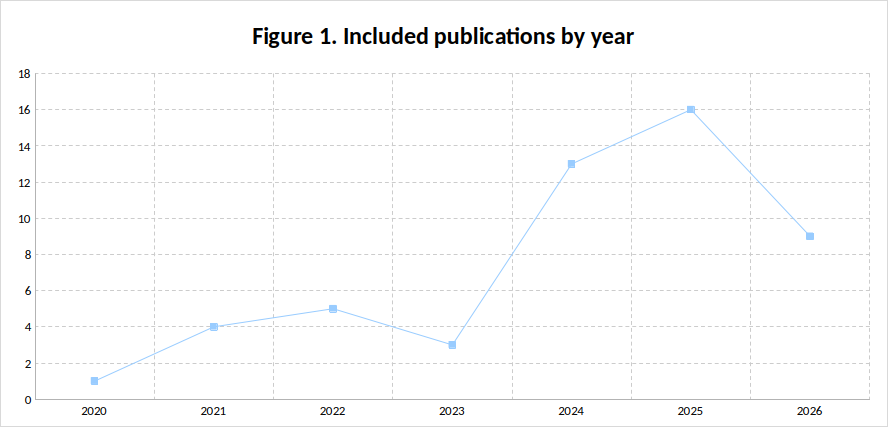
\includegraphics[width=\columnwidth]{figures/fig1.png}
    \caption{Annual distribution of the included DECT-2020 NR publications.}
    \label{fig1}
\end{figure}
\begin{figure}[!t]
    \centering
    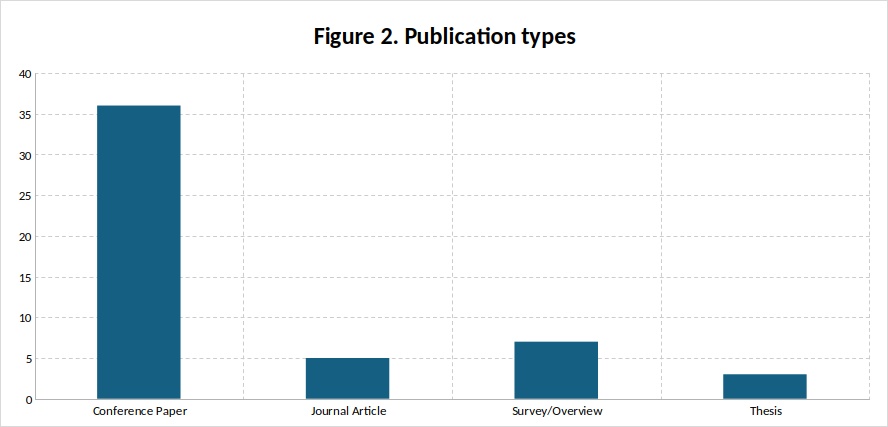
\includegraphics[width=\columnwidth]{figures/fig2.png}
    \caption{Annual distribution of the included DECT-2020 NR publications.}
    \label{fig2}
\end{figure}
\begin{figure}[!t]
    \centering
    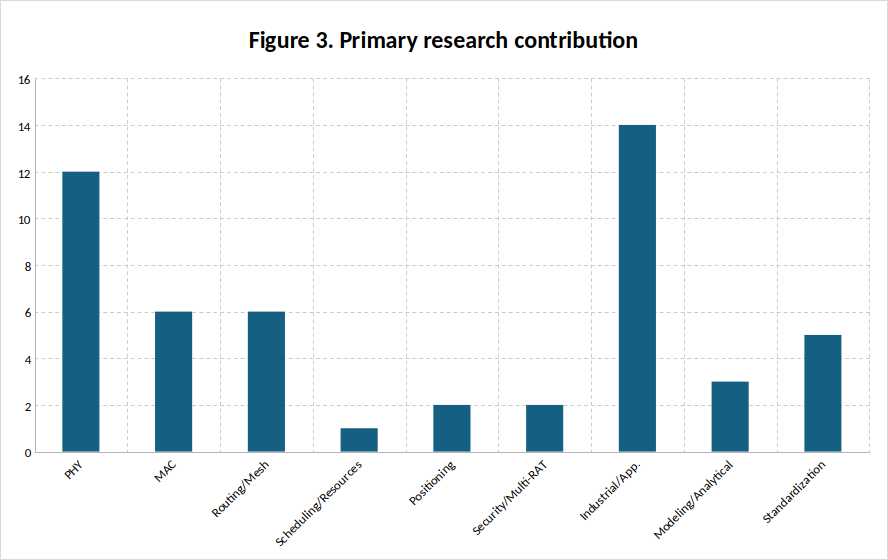
\includegraphics[width=\columnwidth]{figures/fig3.png}
    \caption{Annual distribution of the included DECT-2020 NR publications.}
    \label{fig3}
\end{figure}
\begin{figure}[!t]
    \centering
    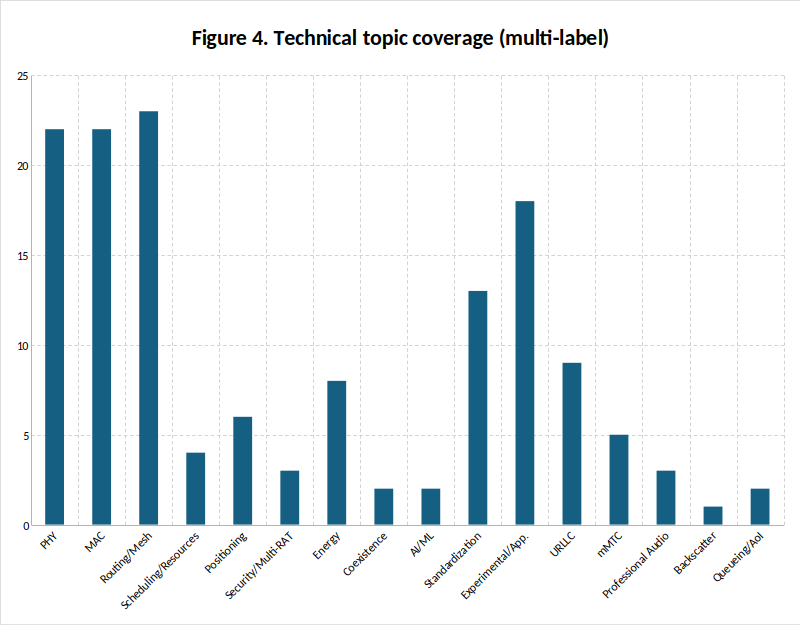
\includegraphics[width=\columnwidth]{figures/fig4.png}
    \caption{Annual distribution of the included DECT-2020 NR publications.}
    \label{fig4}
\end{figure}
\begin{figure}[!t]
    \centering
    
\includegraphics[width=\columnwidth]{figures/fig5.png}
    \caption{Annual distribution of the included DECT-2020 NR publications.}
    \label{fig5}
\end{figure}
\begin{figure}[!t]
    \centering
    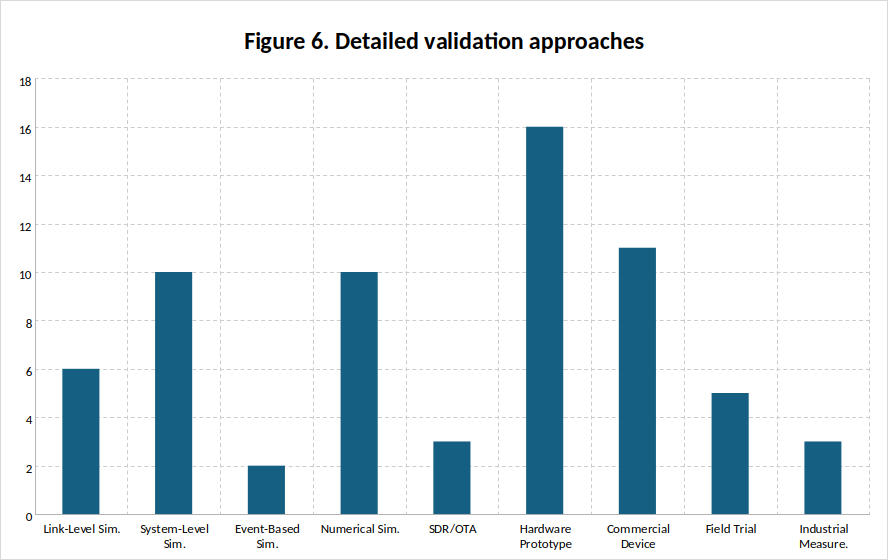
\includegraphics[width=\columnwidth]{figures/fig6.png}
    \caption{Annual distribution of the included DECT-2020 NR publications.}
    \label{fig6}
\end{figure}
\begin{figure}[!t]
    \centering
    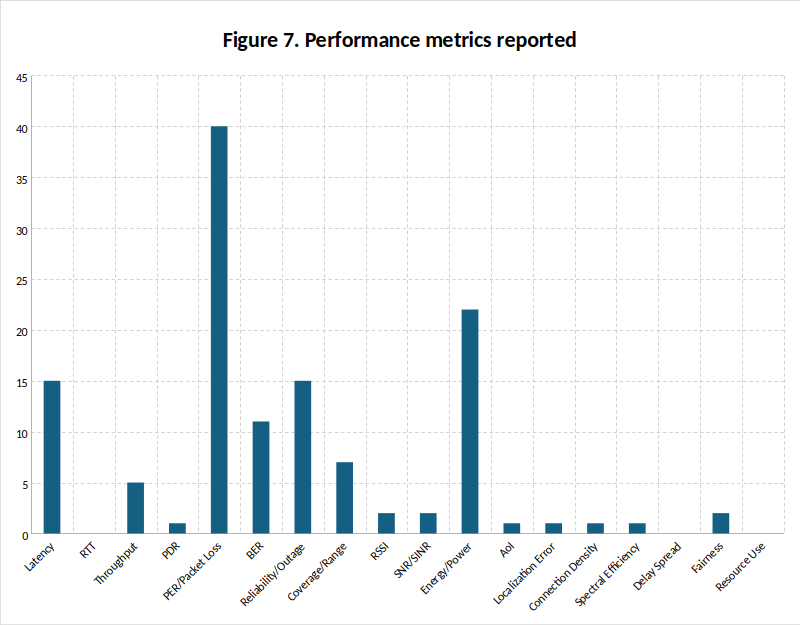
\includegraphics[width=\columnwidth]{figures/fig7.png}
    \caption{Annual distribution of the included DECT-2020 NR publications.}
    \label{fig7}
\end{figure}
\begin{figure}[!t]
    \centering
    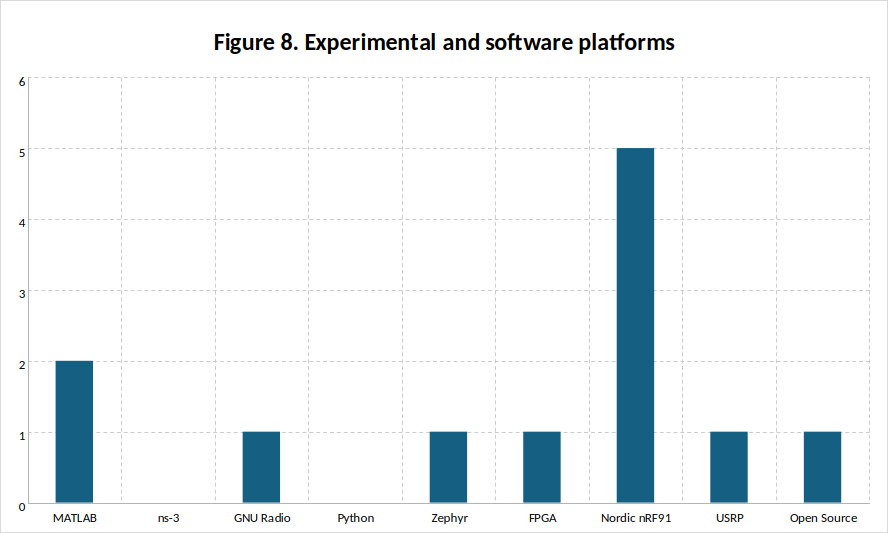
\includegraphics[width=\columnwidth]{figures/fig8.png}
    \caption{Annual distribution of the included DECT-2020 NR publications.}
    \label{fig8}
\end{figure}